\section{CellROX\texttrademark~assay}
\begin{figure}[H]
    \capstart
    \centering
    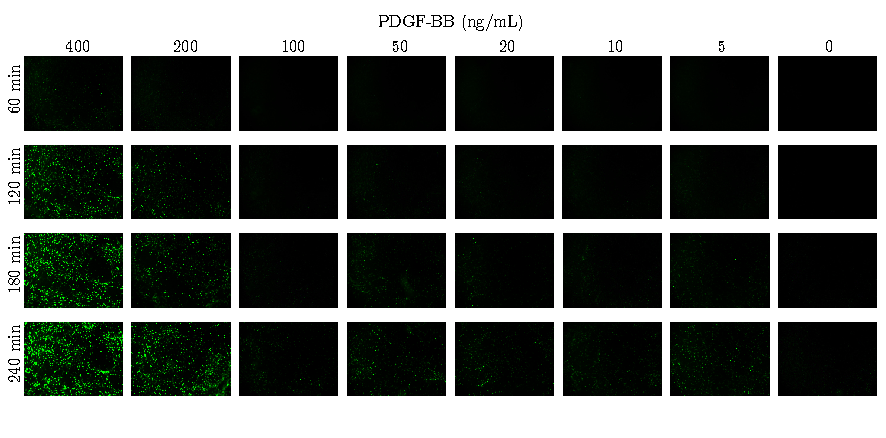
\includegraphics{Abbildung/cellrox_titration_wells_example.pdf}

    \begin{minipage}{\captionwidth}
        \caption[cell_rox_cells]{\uzlemph{Representative CellROX\texttrademark~Green signal for \ac{pdgf} titration}\newline
        }
        \label{fig:cell_rox_cells}
    \end{minipage}
\end{figure}

\section{Evaluation of oxidative stress with an anti-8-oxoguanine antibody}
\subsection{Antibodies}
\begin{longtblr}[]{
    colspec = {X|X|X},
    rowhead = 1
}
    \textbf{Name}                            & \textbf{Species} & \textbf{Manufacturer}    \\ \hline
    Anti-8-Oxoguanine\newline Antibody, clone 483.15 & mouse   & \SigmaA \\
    Alexa Flour\texttrademark~568\newline anti-mouse IgG (H+L)   & donkey       & \Invitrogen
\end{longtblr}

\pagebreak

\subsection{Chemicals}
\begin{longtblr}[]{
    colspec = {X|X},
    rowhead = 1
}
    \textbf{Name} &  \textbf{Manufacturer} \\ \hline
    Acetone      & \Roth            \\
    \acs{dapi}          & \SigmaA            \\
    Methanol ($\geq$99\,\%)      & \Roth            \\
    Trition\textsuperscript{\textregistered} X-100 & \Thermo
\end{longtblr}

In \ac{if} flourescently labeled antibodies are used to specifically target and label a molecule in a biological sample. An anti-8-oxoguanine antibody was used as a complementary approach to CellROX\texttrademark~assay. 8-oxoguanine is a common base lesion that is caused by the oxidation of guanine in the presence of \ac{ros} \cite{leon8OxoguanineAccumulationMitochondrial2016}.\\
For the assay, \acp{haosmc} differentiated according to section \ref{subsec:differentiation} on \ac{col1} matrix were washed with \ac{pbs} and boosted for 90\,min with 500\,mL \ac{M231} supplemented with 1\,\% \ac{fbs} and 200\,ng/mL \ac{pdgf}. After, the cells were fixated with 200\,µL methanol (1:1, -\,20\,°C) for 40\,min. The methanol:aceton was removed and cells were dried for 20\,min. For permeabilization, the cells were incubated with 250\,µL 0.2\,\% Triton\textregistered X-100, 1,\% \ac{bsa} (in \ac{pbs}) for 30\,min. Further, unspecific binding sites were blocked with 250\,µL 3.5\,\% \ac{bsa} (in \ac{pbs}) for 30\,min. Afterward, \acp{haosmc} were incubated with 500\,µL of the primary antibody (1:500 in \ac{pbs}) at 4\,°C over night. In the morning the cells incuabed with 500 µL AF555 anti mouse (1:1000 in \ac{pbs}) and nuclei were stained with \acf{dapi} (1:5000) for 1\,h.

\setcounter{figure}{1}
\begin{figure}[H]
    \capstart
    \centering
    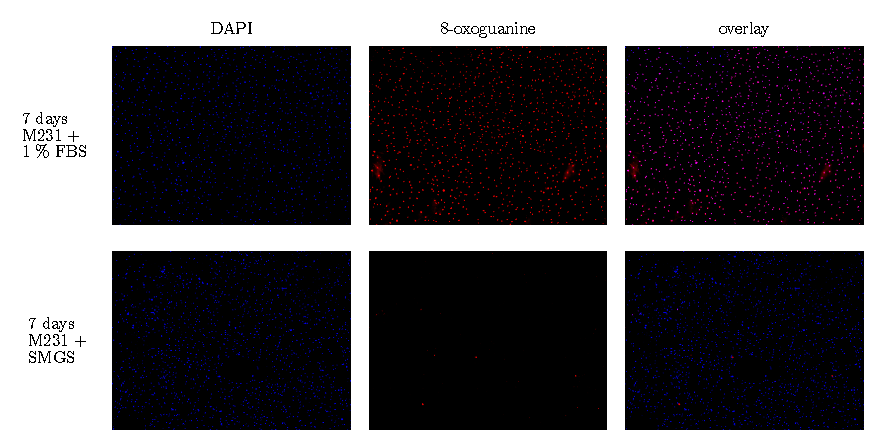
\includegraphics{Abbildung/8oxoG.pdf}

    \begin{minipage}{\captionwidth}
        \caption[antibody]{\uzlemph{Evaluation of oxidative stress with an anti-8-oxoguanine antibody}\newline
        }
        \label{fig:antibody}
    \end{minipage}
\end{figure}

Unfortunately, this approach was unsuccessful, because, as seen in figure \ref{fig:antibody}, starvation of \acp{haosmc} in \ac{M231} supplemented with 1\,\% \ac{fbs} was oxidation of guanine.
